%%%%%%%%%%%%%%%%%%%%%%%%%%%%%%%%%%%%%%%%%%%%%%%%%%%%%%%%%%%%%%%%%%%%%%%%%%%%%% %%
%12345678901234567890123456789012345678901234567890123456789012345678901234567 89
%        1         2         3         4         5         6         7 8

\documentclass[letterpaper,10pt,conference]{ieeeconf}  % Comment this line out if you needa4paper
\usepackage{amsmath}
\usepackage{amssymb}

%\documentclass[a4paper,10pt,conference]{ieeeconf}        % Use this line for a4 paper

\IEEEoverridecommandlockouts                              % This command is only needed if
                                                          % you want to use the \thanks command

\overrideIEEEmargins                                      % Needed to meet printer requirements.

% See the \addtolength command later in the file to balance the column lengths
% on the last page of the document

% The following packages can be found on http:\\www.ctan.org
\usepackage{graphics} % for pdf, bitmapped graphics files
\usepackage{epsfig} % for postscript graphics files
%\usepackage{mathptmx} % assumes new font selection scheme installed
%\usepackage{times} % assumes new font selection scheme installed
\usepackage{amsmath} % assumes amsmath package installed
%\usepackage{amssymb}  % assumes amsmath package installed

\title{\LARGE \bf
 Learning hierarchical representation of 3D objects
}


\author{Dominik Belter, Marek Kopicki, Jeremy Wyatt% <-this stops a space
% \thanks{}% <-this % stops a space
% \thanks{D. Belter, M. Nowicki and P. Skrzypczy\'nski are with the Institute of Control and 
%  Information Engineering, Poznan University of Technology, ul. Piotrowo 3A 60-965 Pozna\'n, Poland,
%  {\tt\small \{name.surname\}@put.poznan.pl}}%
}


\begin{document}


\maketitle
\thispagestyle{empty}
\pagestyle{empty}


%%%%%%%%%%%%%%%%%%%%%%%%%%%%%%%%%%%%%%%%%%%%%%%%%%%%%%%%%%%%%%%%%%%%%%%%%%%%%% %%
\begin{abstract}
\end{abstract}


%%%%%%%%%%%%%%%%%%%%%%%%%%%%%%%%%%%%%%%%%%%%%%%%%%%%%%%%%%%%%%%%%%%%%%%%%%%%%% %%

\section{Related work}

\section{Learning}


\begin{figure}[t]
 \centering
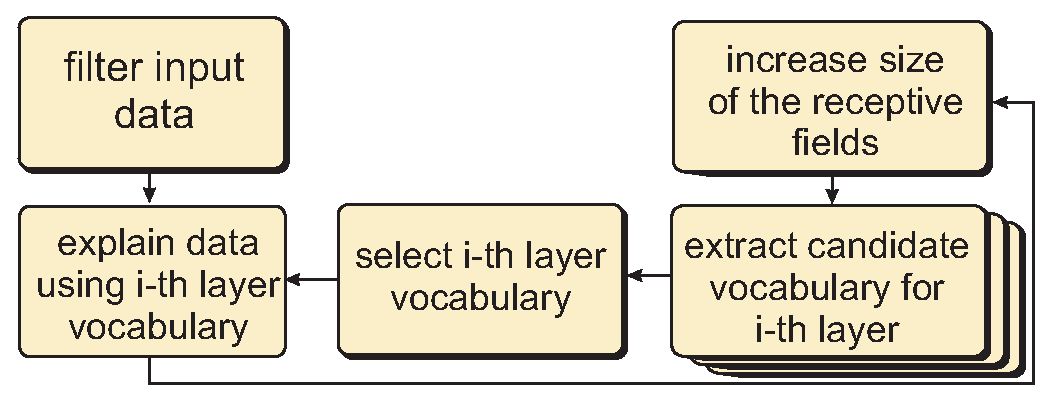
\includegraphics[width=0.9\columnwidth]{../images/learningGeneral.eps}
\caption{General procedure of learning the hierarchical representation of objects}
 \label{hopProc}
\end{figure}

The procedure of learning hierarchical representation of objects is presented in Fig.~\ref{hopProc}. At the beginning, the input data are filtered to remove the noise introduced by the sensor. In the next step the first layer of the hierarchy is defined. Words from the first layer vocabulary are defined over the space of image features. For the grayscale images the Gabor filters might be used~\cite{Fiedler2014}. Each Gabor filter correspond to the edge of the object on the 2D image. Because we create hierarchy from range data the input feature corresponds to the surface of the object and the word in the first layer is represented by the planar patch. 

In the next step of the learning procedure the first layer words (planar patches) are detected on the depth image. Input data is explained using first layer vocabulary. To create next layer vocabulary the size of the receptive field is increased. The words of the $i-th$ layer are created from spatial combination of words of the previous layer. Then, the learning procedure selects representative words for the next layer vocabulary. It allows to reduce the number of words in the vocabulary and to obtain generative properties of the hierarchy. Similar parts are grouped in the same cluster. The whole cluster is represented on the higher level of the hierarchy by the representative part. The representative part might be the part in the center of the cluster. The procedure is repeated the desired number of layers is obtained. In general the size of the receptive field 

\subsection{Implementation}

We learn the hierarchy from range images obtained from Kinect-like sensors. We create two types of vocabularies. First layers of the hierarchy, which are view-dependent, are created using 2.5D depth image. This allows to build representation of the object which is visible from single viewpoint. To build full 3D hierarchical model of the object we build volumetric words in 3D from many depth camera images. 

To create first layer of the hierarchy we remove background from images. Then, we filter the image to remove noise introduced by the sensor. To this end, we applied median filter in 7$\times$7 window. In the hierarchy the first layer is represented by planar patch. According to the general procedure of the hierarchy learning (Fig.~\ref{hopProc}) the next step the input data is explained using first layer vocabulary. Thus we extract planar patches from the depth image. First we compute the normal vector for each point on the image. To compute normal vector we use Principal Component Analysis (PCA). We compute normal using 7$\times$7 window. Because PCA does not work properly on the edges we detect two surfaces inside the sliding window. Then, the points which don't lie on the surface corresponding to the considered point are removed from the patch.

\begin{figure}[t]
 \centering
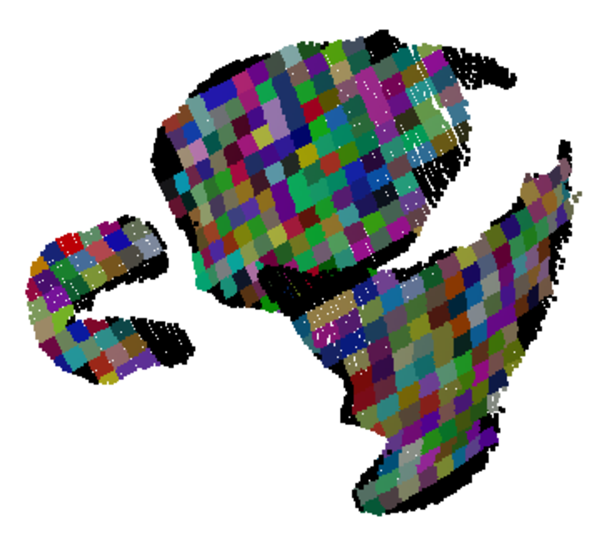
\includegraphics[width=0.5\columnwidth]{../images/recFields1.eps}
\caption{Point cloud obtained from single camera view divided into first layer receptive fields. Each color represent receptive field. Black points are not used to compute planar patches}
 \label{recFields1}
\end{figure}

To extract planar patches from the depth image we divide image space into regular grid. Each cell (5$\times$5 patch) correspond to the receptive field. The surface of the object divided into receptive fields is presented in Fig.~\ref{recFields1}. Inside each receptive field the point which represent planar patch is found. To remove outliers the points are grouped according to the normal vector. For the most numerous group we compute mean normal vector and central position of the patch.

\begin{figure}[t]
 \centering
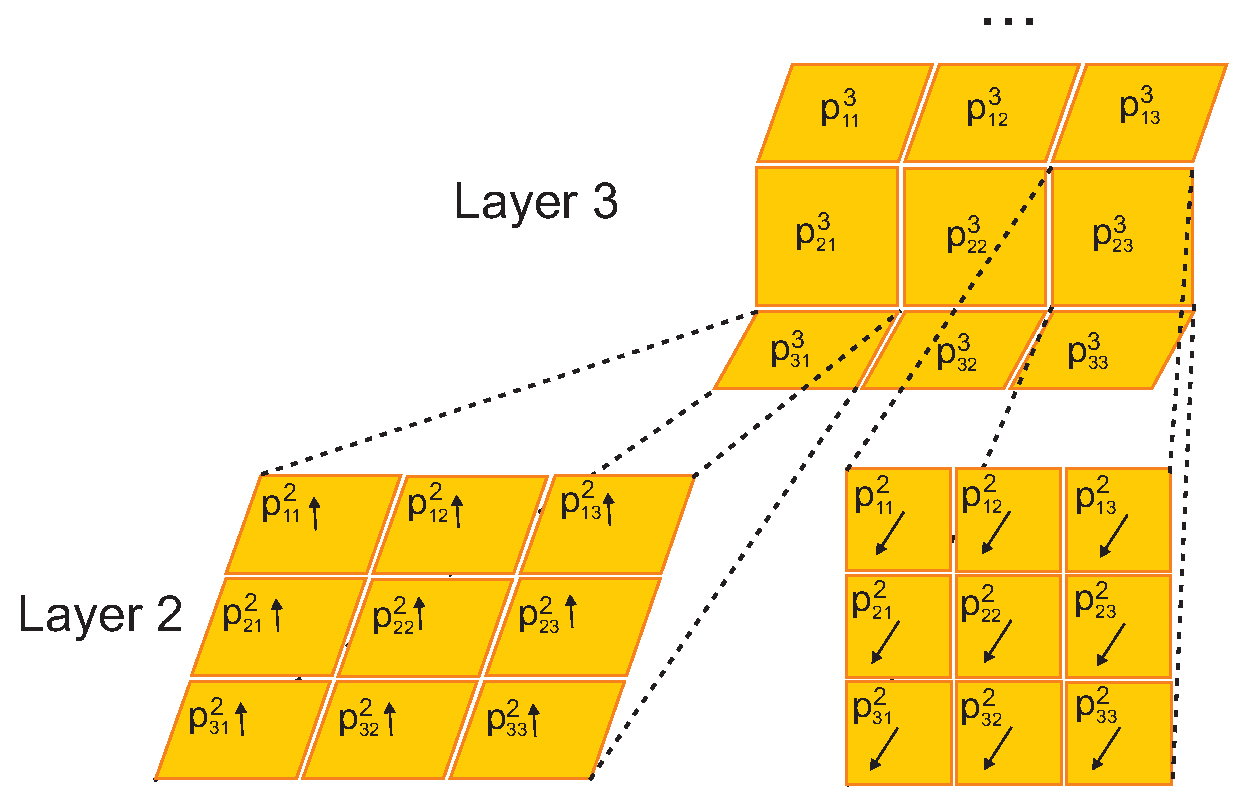
\includegraphics[width=0.9\columnwidth]{../images/word.eps}
\caption{Representation of words in the view-variant layers}
 \label{word}
\end{figure}

The next layer vocabulary is formed on the image plane. To create words of the $l+1$ layer the size of the receptive field is increased. The procedure is presented in Fig.~\ref{word}. The receptive field of the $l+1$ layer covers nine receptive fields of the $l$-th layer. The second layer's word contains maximally nine planar patches. If the receptive fields does not cover the surface of the object the sub-part is represented by the background. The minimal number of sub-parts in the second layer word (part) is set to four. This is the minimal number of points required to compute similarity between parts.

The words of the second layer are extracted from all images used for training the hierarchy. The variability of the words used for learning is increased by introduction overlapping receptive fields. Overlapping receptive fields allows also to deal with the problem related to the division of the image into regular grid. The position of the camera in relation to the object strongly influence the position of the receptive fields on the objects surface. The problem exists on the edges of the object. If the receptive field is shifted the part computed for the surface may overlap the object, the background or both. The position of the receptive field influences the part detected on the image. By applying overlapping receptive field the number of hypothesis about the point on the image plane is increased.

\begin{figure}[t]
 \centering
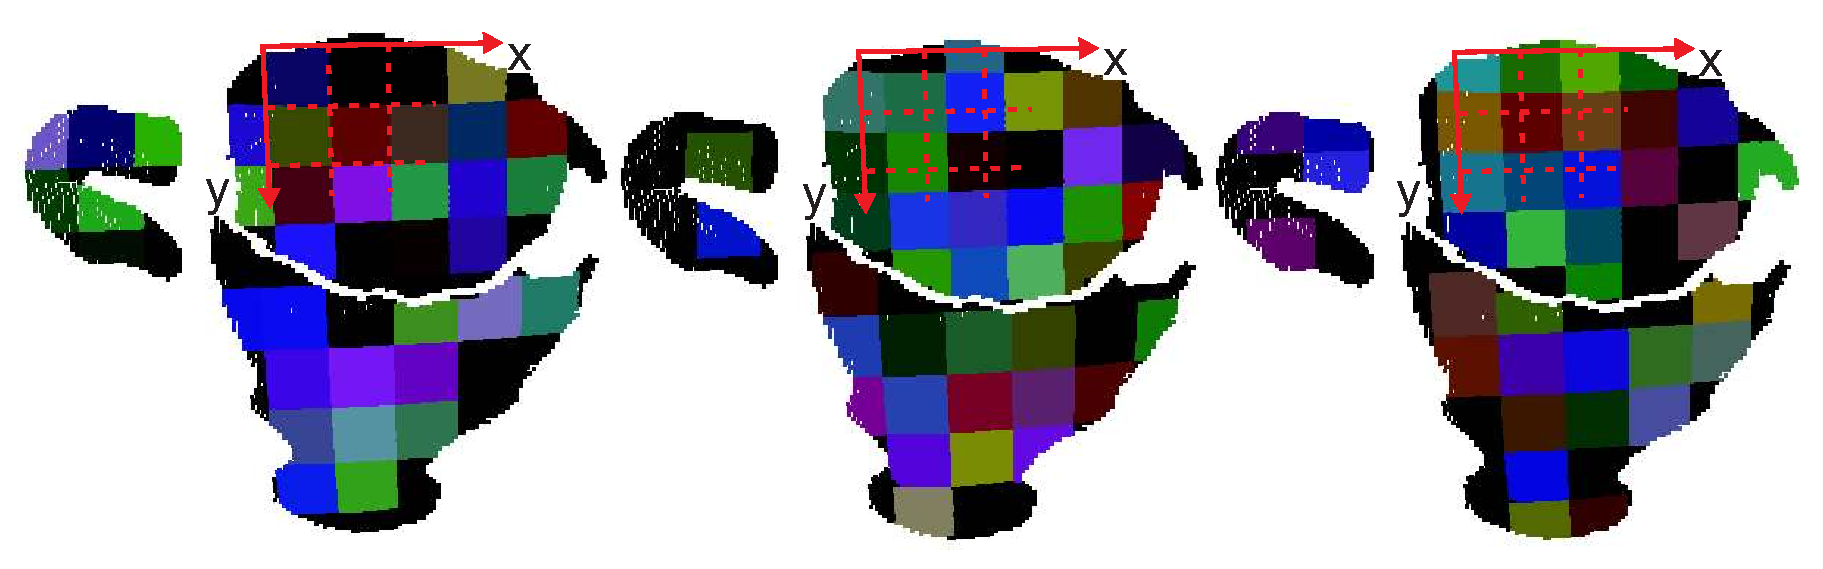
\includegraphics[width=0.99\columnwidth]{../images/overlap.eps}
\put(-222,62){a} \put(-142,62){b} \put(-60,62){c}
\caption{Overlapping receptive fields: receptive field shifted by 0\% (a), 33\% (b) and 66\% (c)}
 \label{overlap}
\end{figure}

The overlapping receptive fields are presented in Fig.~\ref{overlap}. The overlapping receptive field is moved by the width of the $l-1$ part (33\% and 66\% of the $l-th$ layer part). It means that each point on the image might be explained by three different parts.

In the next step of the learning procedure the candidate vocabulary for i-th layer is extracted. Words obtained from all depth images and for all overlapping receptive fields are selected. Then, we select the next layer vocabulary by clusterization of parts (words) in the vocabulary. To this end, the hierarchical agglomerative clustering is used~\cite{Manning2008}. We merge clusters according to the similarity between parts. We stop the procedure if the distance (similarity) between parts $d^c$ is bigger than threshold. Moreover, after each step which merges two clusters we compute maximal distance $d^c_{\rm max}$ between parts inside the cluster. If the distance inside the cluster is bigger than threshold the cluster is splited into two separate clusters. By using this procedure we accept maximal error between parts inside cluster. The number of obtained parts in the vocabulary depends on two parameters: $d^c$ and $d_{\rm max}$.

To compute similarity between two view dependent parts $p_A$ and $p_B$ we defined the distance metric $d_{\rm VD}$:

\begin{equation}
\label{distVD}
 d_{\rm VD}=\sum_{i,j}^N ( c_1 d(p_A^{\rm ij}, p_B^{\rm ij}) + c_2 {\bf N}_A^{\rm ij} \cdot {\bf N}_B^{\rm ij}),
\end{equation}

where $d(p_A^{\rm ij}, p_B^{\rm ij})$ is the Euclidean distance between centers of corresponding patches, $N_A^{\rm ij}$ and $N_A^{\rm ij}$ are corresponding normal vectors in part A and B, $c_1$ and $c_2$ are constant values which scale Euclidean distance and dot product between normal vectors. The distance $d_{\rm VD}$ is computed taking into account corresponding sub-part. If both sub-parts are background the distance value is not increased. If one of the corresponding sub-part is background and second corresponds to planar patch the distance $d_{\rm VD}$ is increased by constant value $c_3$.

Despite of the fact that first layers of the hierarchy are view-dependent we store in the hierarchy parts which are view-invariant. It means that that we can distinguish between planar, concave, convex and other part independently from the angle of observation. It allows to reduce significantly the number of parts which are stored in the hierarchy. In contrast to hierarchy presented for 2D images~\cite{Fiedler2014} the discretization of normal vectors is not required in hierarchy of 3D parts. We store continues values of the normal vector. We can also learn hierarchy from few examples. Single camera image provides multiple realizations of parts. If parts are view-variant the number of learning examples should be significant to provide sufficient statistics for learning. In this case objects should be observed from multiply viewpoints.

To obtain view invariance of parts we solve optimization problem:

\begin{equation}
\label{optVI}
 \arg\min_{\bf T} d_{\rm VD}({\bf T}),
\end{equation}

where ${\bf T}$ is special Euclidean group SE(3) rigid body transformation, $d_{\rm VD}({\bf T})$ is the distance metric (\ref{distVD}) computed for part $p_A$ and part $p_B$ transformed by ${\bf T}$. To find the rigid body transformation ${\bf T}$ which aligns part A and part B we use Umeyama method~\cite{Umeyama1991}. Umeyama methods finds optimal transformation ${\bf T}$ (root mean squared error is minimized) between points with known correspondence. To find correspondences between patches in parts we perform exhaustive search. We take into account 8 possible rotations of parts around central element. Note that we don't rotate part in 3D space. We modify correspondences between elements only. After this step the parts are aligned by Umeyama method and the similarity distance $d_{\rm VD}({\bf T})$ between parts is computed. 

\begin{figure}[t]
 \centering
 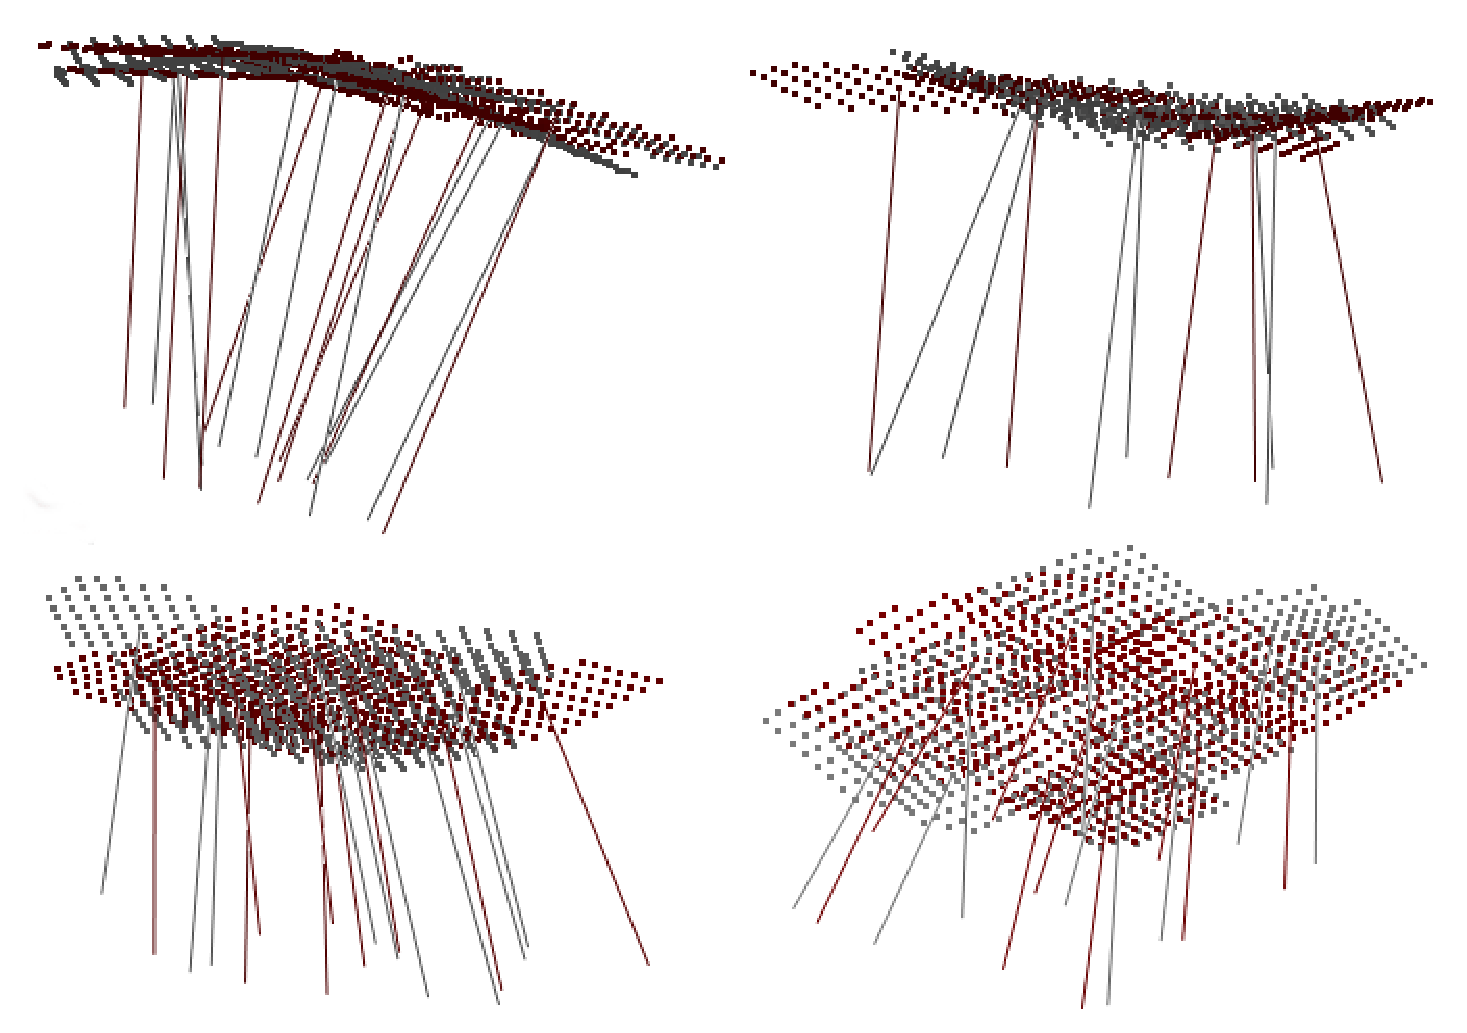
\includegraphics[width=0.95\columnwidth]{../images/parts2ndLayer.eps}
 \caption{Alignment of parts from the second layer. Gray -- part A ($p_A$), red -- part B ($p_B$)}
 \label{parts2ndLayer}
\end{figure}

To align parts from the the $l$-th layer the hierarchical structure of parts has to be used. Parts of higher layers are created from parts of the lower layers. To obtain point cloud, find correspondences and compute optimal alignment the subparts have to be recursively represented by points with normal vectors. Thus, the part of the first layer are represented by single point, part of the second layer is represented by 9 points, third layer part by 81 points, size $s_{\rm l+1}$ of the $l+1$ layer part is $9s_l$. 

The example alignment for parts from second layer is presented in Fig.~\ref{parts2ndLayer}. We represent each planar patch as a point cloud. The parts does not match perfectly. Small differences in position of subparts and their orientation and even missing sub-part are acceptable. This property enables the capability of the hierarchy to generalize learned models and classify parts properly despite of the sensor noise. 

\begin{figure}[t]
 \centering
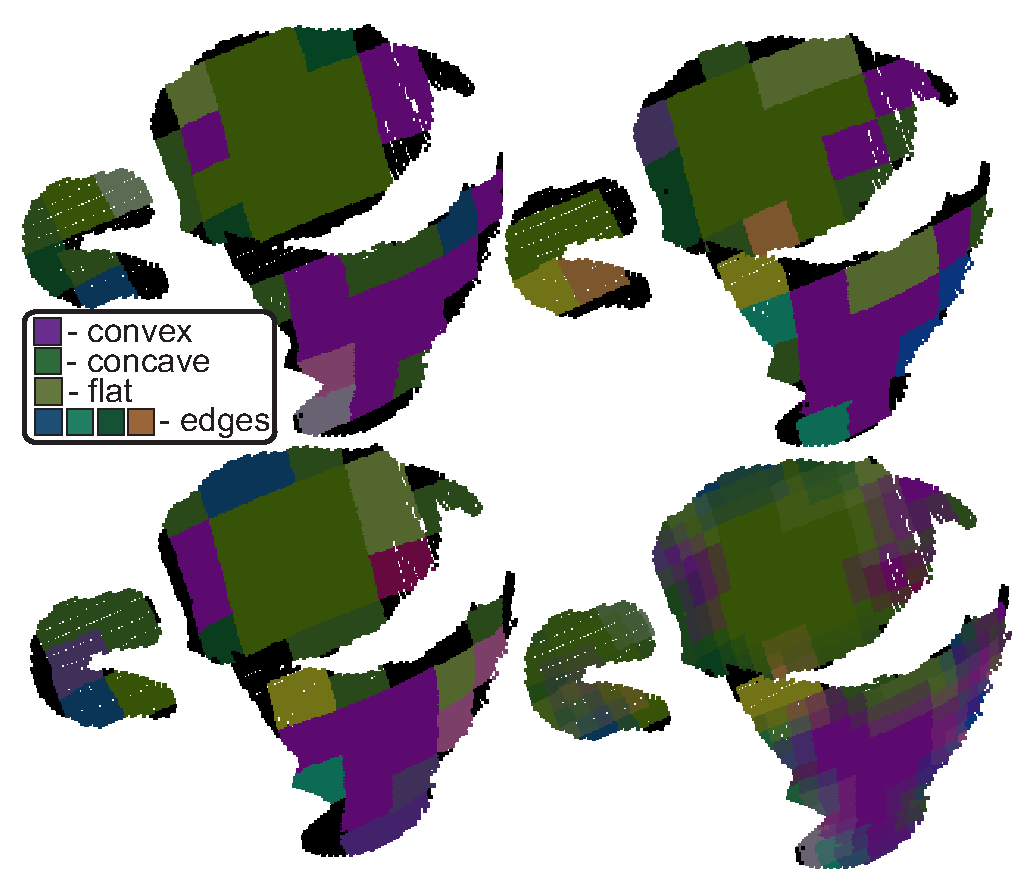
\includegraphics[width=0.95\columnwidth]{../images/2ndLayer.eps}
\put(-215,182){a} \put(-102,182){b}
\put(-215,82){c} \put(-102,82){d}
\caption{Clusterization results for the second layer. Parts from the same group have the same color on the object visualization: overlap 0\% (a), overlap 33\% (b), overlap 66\% (a), combination of hypotheses (d)}
 \label{2ndLayer}
\end{figure}

The variability of subparts is encoded in the clusters. Clusters are created without supervision. The algorithm can properly generate group of planar, concave and convex parts. Other groups contain various elements which represent edges on the depth image. These parts contain sub-parts created from planar patches and background. The example clusterization results for overlapping receptive fields and single camera view are presented in Fig.~\ref{2ndLayer}. The hierarchy can distinguish between various parts and group them if the local shape is similar. Some surface are misclassified. The size of the receptive field in the second layers is small and the noise of the sensor plays important role here. However, the multiple hypothesis about the parts help to deal with this problem (Fig.~\ref{2ndLayer}).  

\subsection{data explanation using $l$-th layer vocabulary}

\begin{figure}[t]
 \centering
\includegraphics[width=0.95\columnwidth]{../images/explanation2ndLayer.eps}
\put(-232,172){a} \put(-232,77){b}
\caption{Explanation of data using vocabulary from second layer without (659 parts) (a) and with compression (38 parts) (b)}
 \label{explanation2ndLayer}
\end{figure}

In the next step the input data is explained using the obtained $l$-th layer vocabulary. We explain the image using representative parts only. Thud, some areas of the image are replaced by $l$-th layer representative parts. This enables the compression of the input data as well as generalization. Using information about camera pose the parts can be moved into 3D space and reconstruct the object. Then, we can check visually the compression and clusterization results. The obtained representation of the object created from second layer vocabulary is presented in Fig.~\ref{explanation2ndLayer}. In Fig.~\ref{explanation2ndLayer}a the object created from 659 parts is presented. In this case the compression rate is set to 0\%. In Fig.~\ref{explanation2ndLayer}b the objects is created from 38 parts only. The compression rate for this layer is 5.8\%. Despite of the high reduction of parts the explanation of the input data is still precise. Moreover, the normal angles are more smooth for the object created from compressed vocabulary. This property is comes out from the clusterization. The variation of the shape  inside clusters which caused also by the sensor noise is represented by the ``average'' part in the center of the cluster.

\begin{figure}[t]
 \centering
 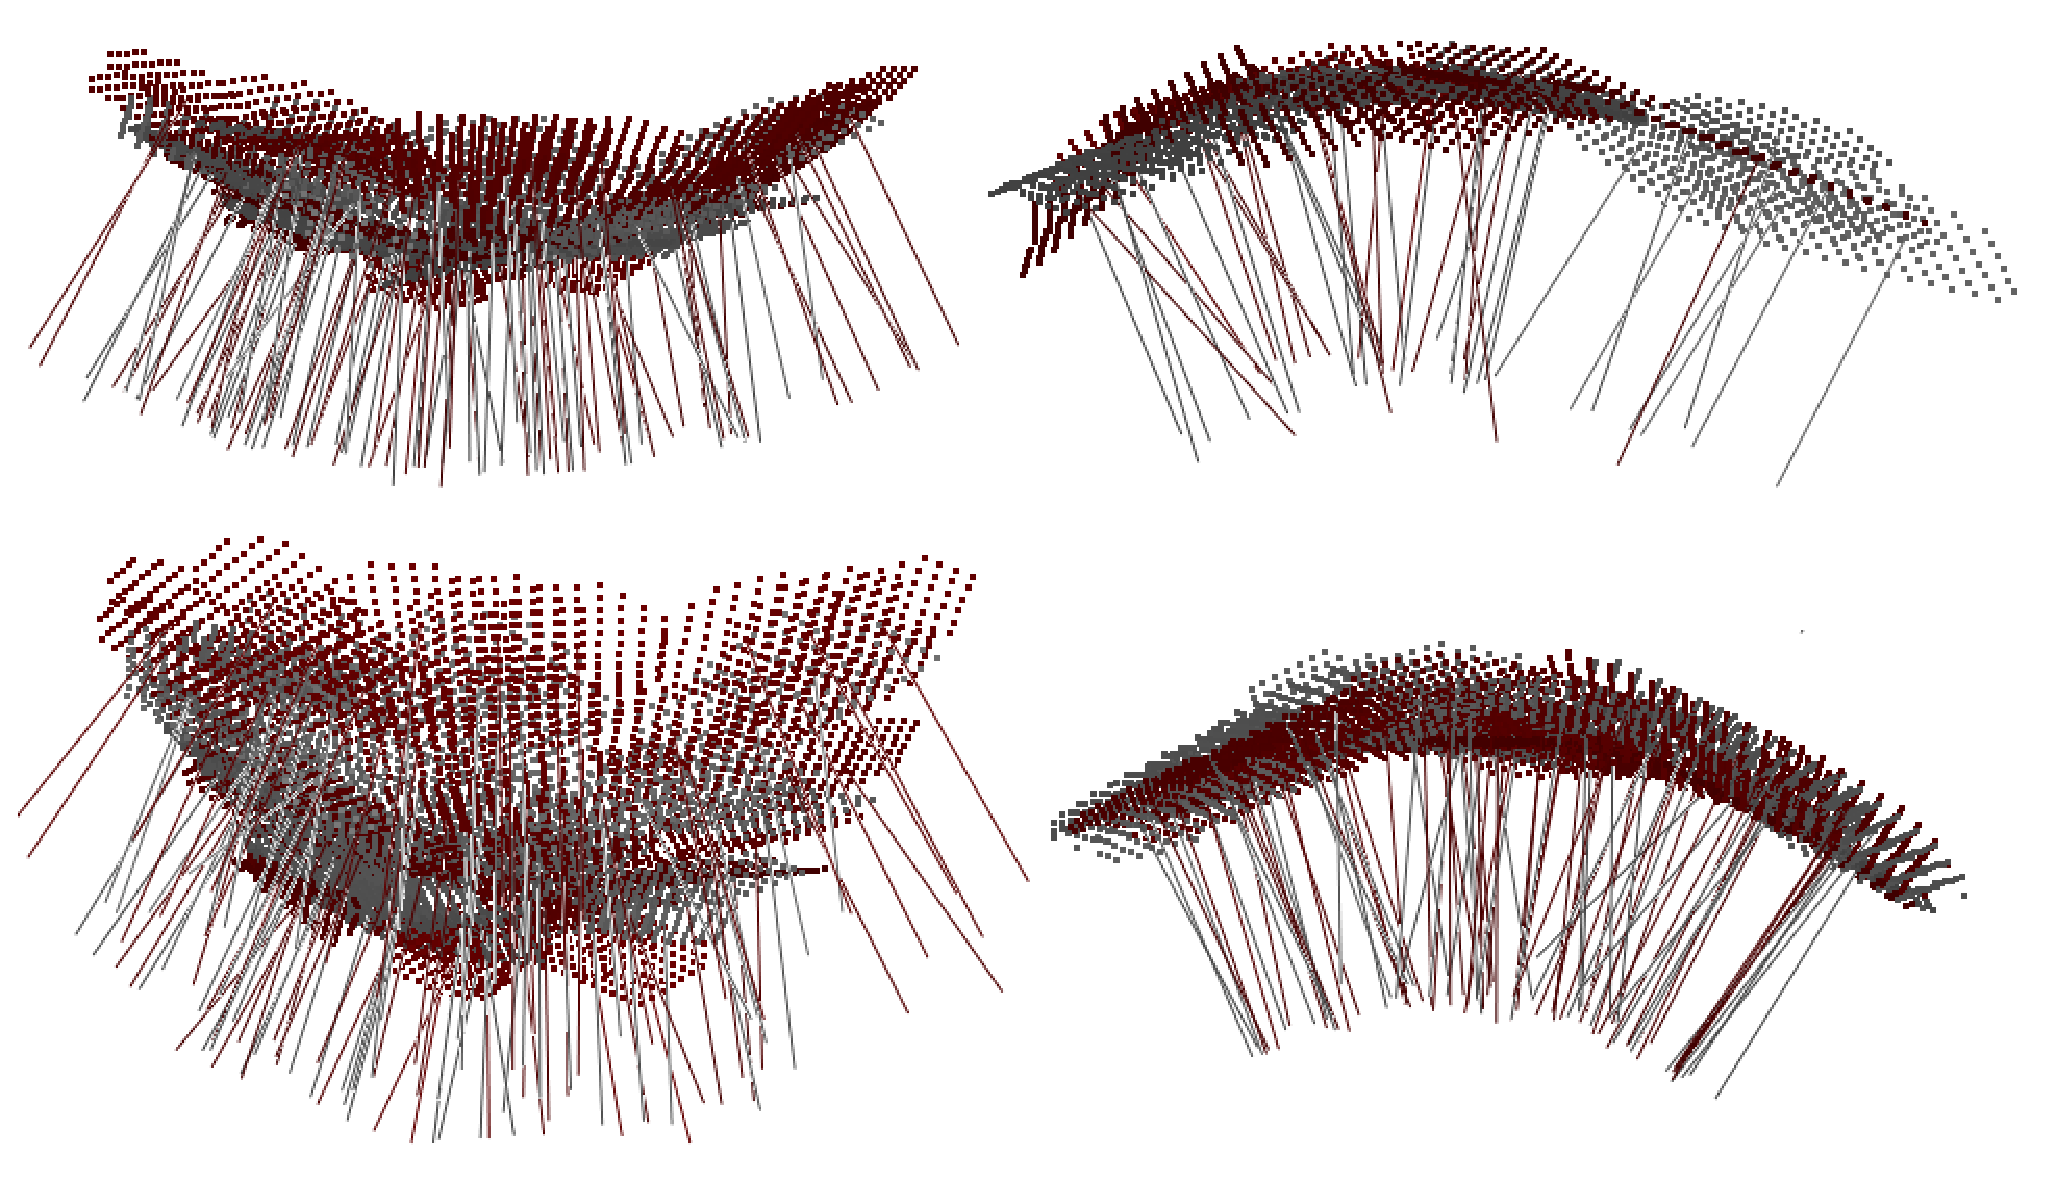
\includegraphics[width=0.95\columnwidth]{../images/parts3rdLayer.eps}
 \caption{Alignment of parts from the third layer. Gray -- part A ($p_A$), red -- part B ($p_B$)}
 \label{parts3rdLayer}
\end{figure}

\begin{figure}[t]
 \centering
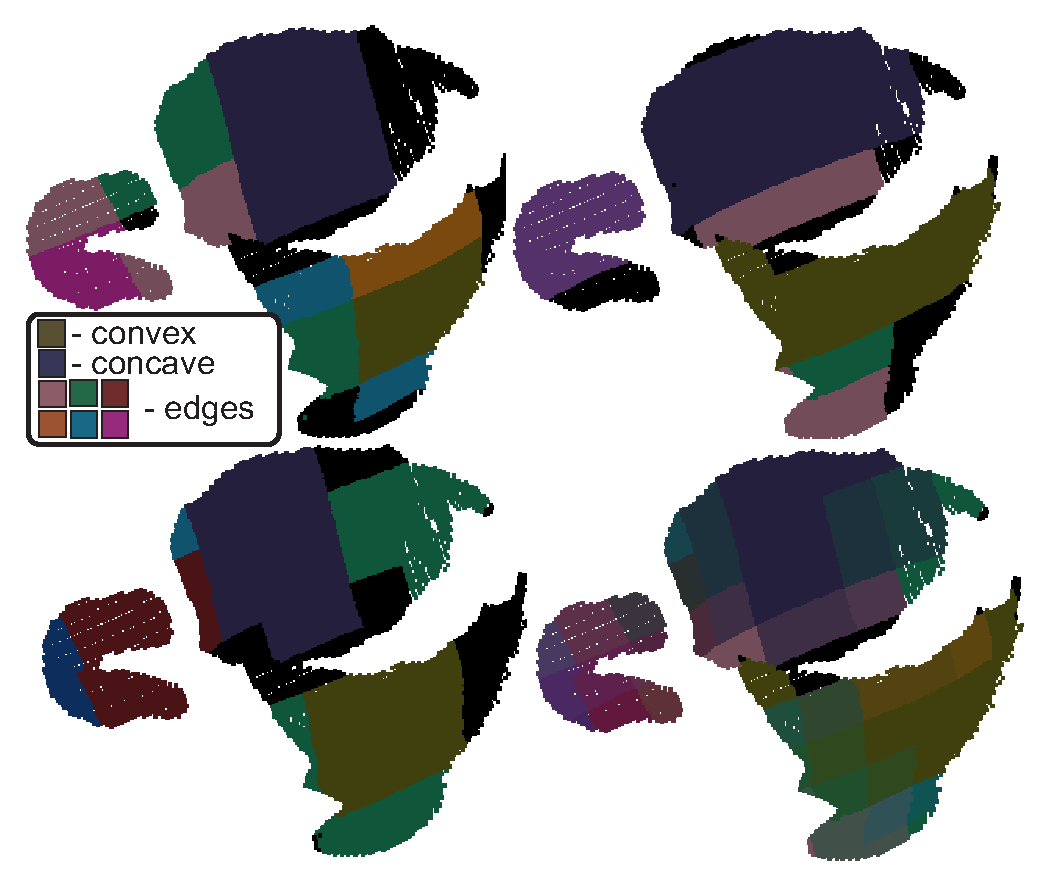
\includegraphics[width=0.95\columnwidth]{../images/3rdLayer.eps}
\put(-215,182){a} \put(-102,182){b}
\put(-215,82){c} \put(-102,82){d}
\caption{Clusterization results for the second layer. Parts from the same group have the same color on the object visualization: overlap 0\% (a), overlap 33\% (b), overlap 66\% (a), combination of hypotheses (d)}
 \label{3rdLayer}
\end{figure}

\begin{figure}[t]
 \centering
\includegraphics[width=0.95\columnwidth]{../images/explanation3rdLayer.eps}
\put(-232,172){a} \put(-232,77){b}
\caption{Explanation of data using vocabulary from third layer without (143 parts) (a) and with compression (36 parts) (b)}
 \label{explanation3rdLayer}
\end{figure}

The procedure of learning $l$-th layer vocabulary is repeated for view-dependent layers until the desired number of layers is obtained. The obtained alignment of parts in the third layer is presented in Fig.~\ref{parts3rdLayer}. The obtained clusters are presented in Fig.~\ref{3rdLayer}. For the third layer the compression rate is 25.2~\%. For the third layer the obtained compression is significantly smaller than for the second layer. In the third layer the receptive fields are three times bigger than in the second layer (Fig.~\ref{word}). At this size of the receptive field the difference between concave, convex and flat parts is bigger. On the other hand, parts overlapped by receptive fields are more unique and clusterization of parts produces higher number of groups. The higher compression is possible but the higher reconstruction error has to be accepted. The explanation of the input data using third layer vocabulary is presented in Fig.~\ref{explanation3rdLayer}.

\subsection{View-invariant representation of parts}

Parts obtained from single camera view do not provide full information about the shape of the object. It's difficult to conclude about parts which are located on the edges of the object. The system which learns from single view does not have information that some edges visible from a single view correspond to continuous surface of the object. The discrepancy between these parts is important when the robot grasp the object. The grasps that can be attached to the real 3D edge of the object and the edge visible from single camera view are different. Without the knowledge that some edges on 2D image might represent continuous surface the grasping method might fails.

To deal with the proper representation of objects in 3D we build the hierarchy which contains view view-variant and view invariant layers. View-variants layers contain view-invariant parts (the id of the part depend on the local surface of the object and the id should be independent from camera viewpoint) obtained from single camera frame. The parts are created using 2.5D depth image space. The view-invariant layers are created from multiple camera frames in the volumetric space.

\begin{figure}[t]
 \centering
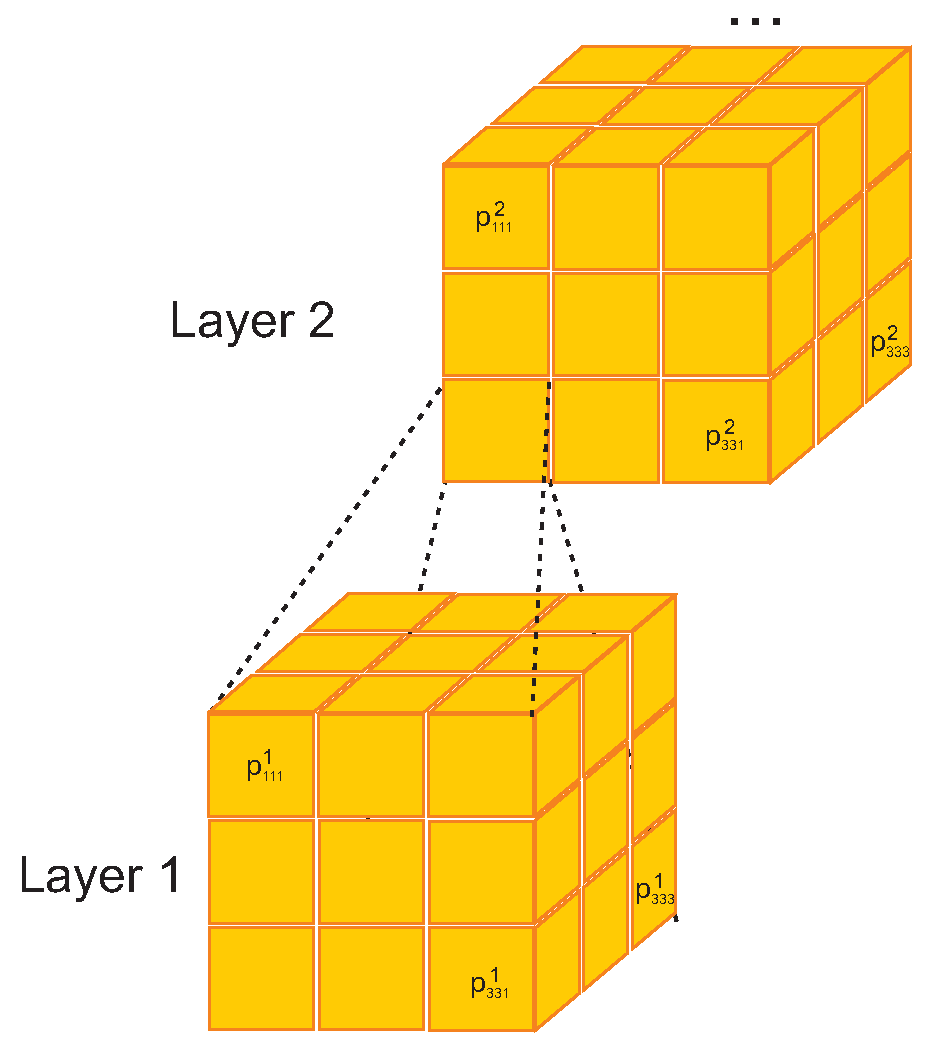
\includegraphics[width=0.75\columnwidth]{../images/wordInd.eps}
\caption{Representation of words in the view-invariant layers}
 \label{wordInv}
\end{figure}

The general learning principle is the same for view-variant and view-invariant layers (Fig.~\ref{hopProc}). For view-invariant volumetric layers the receptive field is represented by the box. The relation between words from $l$ and $l+1$ layers is presented in Fig.~\ref{wordInv}. The word of the $l+1$ layer consists 27 words (parts) from the $l$-th layer. The receptive fields for the volumetric layers grows in three dimensions.

To create first layer of the volumetric vocabulary we transform each part from the view-dependent layer into 3D using known position of the camera for each viewpoint. Then, we hierarchically convert each part into point cloud. We store all points related to each object in separate octree. To reduce number of points and to combine information about surface observed from many viewpoints we run voxel grid filtering~\cite{Aldoma2012}. In contrast to~\cite{Aldoma2012} we preserve normal vectors fro each voxel. During computation of mean point for each voxel the point are clustered according to the normal vector. The maximal distance between normal vectors inside single cluster is set to 45$^\circ$. For each obtained cluster the mean position and normal vector is computed. This approach allows to preserve inner and outer surfaces of the objects.

\begin{figure}[t]
 \centering
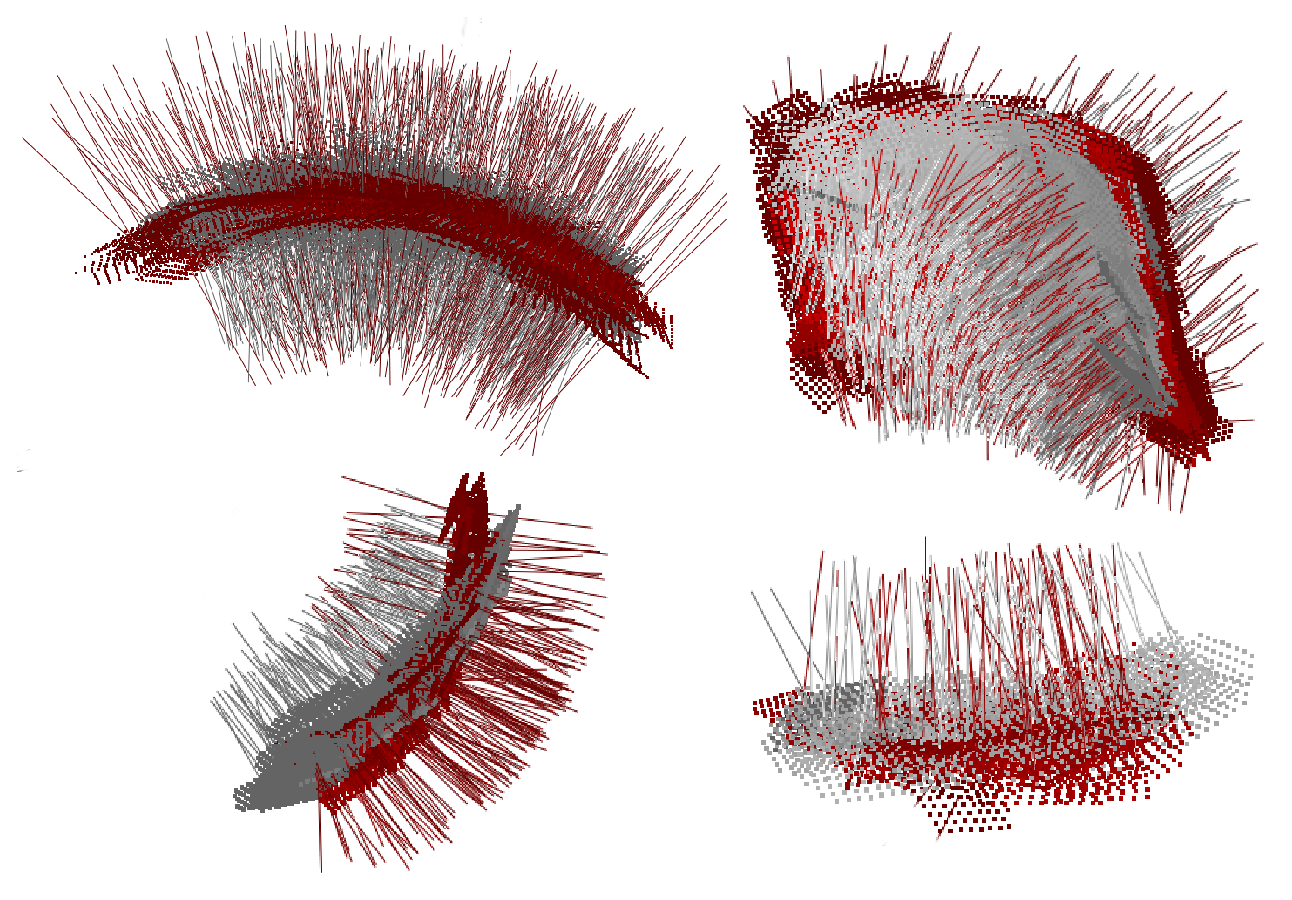
\includegraphics[width=0.95\columnwidth]{../images/viParts.eps}
\caption{Alignment of parts from the fourth layer. Gray -- part A ($p_A$), red -- part B ($p_B$)}
 \label{viParts}
\end{figure}

To compute similarity between view-invariant parts we find the SE(3) transformation $T$ which aligns two parts. To find the optimal transformation $T$ we minimize the error:

\begin{equation}
\label{optVol}
 \arg\min_{\bf T} (n_A-n_B)^2 \sum_i ||{\bf N}_B^i \cdot ({\bf T}\cdot {\bf p}_A^{\rm i}-{\bf p}_B^{\rm i})||^2,
\end{equation}

where ${\bf p}_A^{\rm i}$ and ${\bf p}_B^{\rm i}$ are corresponding points from part A and part B, $n_A$ and $n_B$ are number of points in parts, ${\bf N}_B^i$ is the surface normal at ${\bf p}_B^{\rm i}$. The element $(n_A-n_B)^2$ in (\ref{optVol}) is added to prevent matching parts with significantly different size. To find correspondence between points and to compute optimal transformation $T$ we use point-to-plane variant of Iterative Closest Point~\cite{Segal2009}. To prevent sub-optimal solutions we run ICP multiple times. Each optimization starts from randomly initialized initial guess. Because positions of points in parts are defined in the center of the part we only initialize randomly the orientation of the parts. 

The example alignment of parts from the fourth layer is presented in Fig.~\ref{viParts}. In contrast to parts from view-dependent layers the parts from volumetric layers contain two surfaces. Parts created from single view represent single surface. View invariant parts from volumetric layers represent inner and outer surfaces of the objects (cf. Fig.~\ref{parts3rdLayer} and Fig.~\ref{parts2ndLayer}).

The procedure parts selection is the same as for view-dependent layer. When the next layer vocabulary is selected the receptive fields are increased and the part extraction procedure is repeated (Fig.~\ref{hopProc}). To minimize the influence of the object pose in relation to the global coordinate system the view-invariant receptive fields are also shifted by 33\%. This strategy also provides redundant information about parts covered by receptive fields. Thus, the identification of parts for grasping is more robust.

\section{Results}

\begin{figure}[t]
 \centering
\includegraphics[width=0.95\columnwidth]{../images/shareability.eps}
\put(-227,420){a} \put(-110,420){b}
\put(-227,325){c} 
\put(-227,160){d} 
\caption{Shareablity of parts from view-dependent layers between two categories of objects (bowl (a) and mug (b)) for: second (c) and third (d) layer parts of the hierarchy}
 \label{shareability}
\end{figure}

The learning of the hierarchy allows o find parts which explain the input data. The most important property oh the hierarchy is shareability. The parts are shared between object thus the grasp can be also transfered from the training object to another object. The shareability of parts from view-dependent layers is presented in Fig.~\ref{shareability}. The shareability is presented for two types of objects: mug and bowl. In Fig.~\ref{shareability}c parts from second layers are presented. The parts which represent concave surface (green) can be found on the surface mug which is visible from two various viewpoints as well as on the inner surface of the bowl. Convex parts (pink) are mainly visible on the outer surface of the mug. Some realizations of convex parts can be also found on the bowl's surface but they only represent local shape of the surface.

Shareability of parts is also visible on the 3rd layer of the hierarchy (Fig.~\ref{shareability}c). Because the size of the receptive field is bigger the difference between geometric properties of the surface (convex and concave) are clearly visible. The same parts realizations can be found on the surface of the mug and on the surface of the bowl (concave parts represented by purple color).

\begin{figure}[t]
 \centering
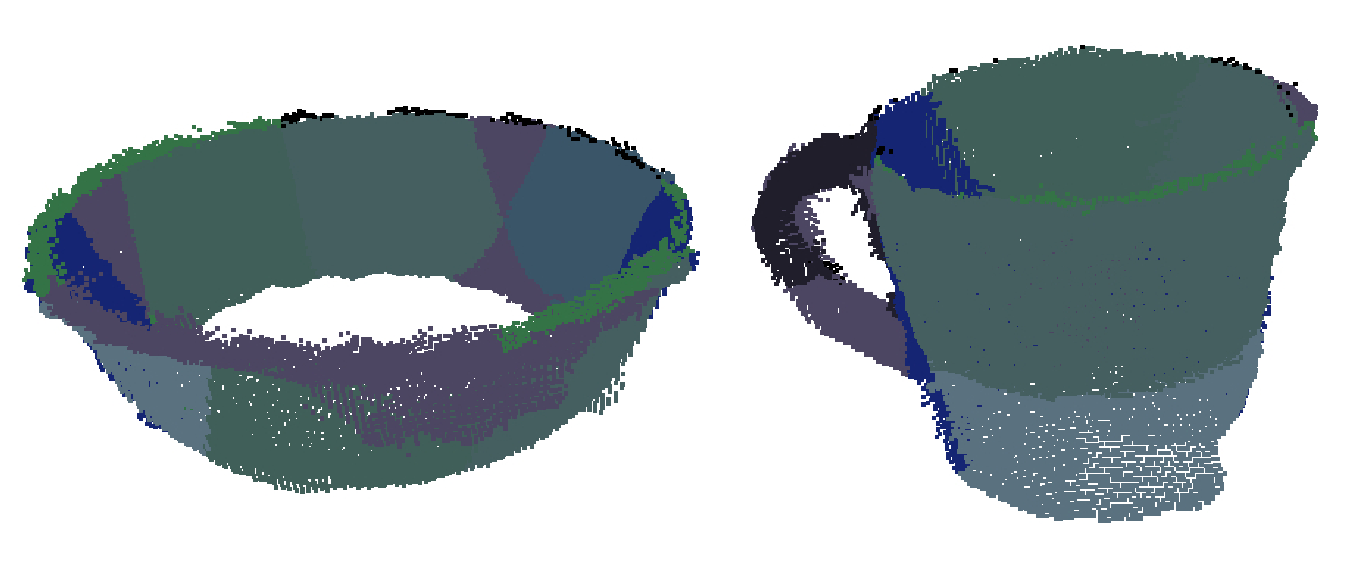
\includegraphics[width=0.95\columnwidth]{../images/shareability4thLayer.eps}
\put(-227,80){a} \put(-100,80){b}
\caption{Shareablity of 4th layer parts between objects}
 \label{shareability4thLayer}
\end{figure}

The shareability of parts can be also observed in volumetric layers of the hierarchy (Fig.~\ref{shareability4thLayer}). Some parts representing edges (green and purple) as well as bigger parts which correspond to inner and outer surface of the object are shared between mug and bowl. Note that some parts which are related to the edges can be also found on the objects surface (purple parts in Fig.~\ref{shareability4thLayer}a). This comes from the regular grid which represent receptive fields. The position of the receptive fields in 3D strongly influence how the object is divided into parts. To mitigate this problem we implemented overlapping receptive fields. The information about spurious edges can be also ignored because the location of the edge is not supported by parts from lower layers of the hierarchy.

\addtolength{\textheight}{-12cm}  

% \section*{APPENDIX}

% Appendixes should appear before the acknowledgment.

% \section*{ACKNOWLEDGMENT}
% acknowledgment

\begin{thebibliography}{99}
\bibitem{Aldoma2012}
A. Aldoma, Z.C. Marton, F. Tombari, W. Wohlkinger, C. Potthast, B. Zeisl, R.B. Rusu, S. Gedikli, M. Vincze, Point cloud library: Three-Dimensional Object Recognition and 6 DoF Pose Estimation. IEEE Robotics \& Automation Magazine, pp.~80-91, 2012
\bibitem{Fiedler2014}
  S. Fidler, M. Boben, A. Leonardis, Learning a Hierarchical Compositional Shape Vocabulary for Multi-class Object Representation, Computer Vision and Pattern Recognition, 2014 (under review)
\bibitem{Umeyama1991}
 S. Umeyama,
 ``Least-squares estimation of transformation parameters between two point patterns'',
 IEEE Trans. on Pattern Analysis \& Machine Intelligence, 13(4), 1991, 376--380.
 \bibitem{Manning2008}
 C. D. Manning, P. Raghavan, H. Sch\"{u}tze, Introduction to Information Retrieval, Cambridge University Press. 2008
 \bibitem{Segal2009}
 A. V. Segal, D. Haehnel, and S. Thrun, Generalized-ICP, Robotics: Science and Systems, 2009
\end{thebibliography}

\end{document}